\section{Zielsetzung}
\label{sec:Zielsetzung}
Das Ziel dieses Versuches ist sich mit verschiedenen gedämpften und erzwungen Schwingungen innerhalb einer Schaltung
 bestehend aus Widerständen, Kondensatoren und Spulen, auseinanderzusetzen. Insbesondere wird sich mit einer gedämpften Schwingung, dem aperiodischen 
 Grenzfall und der Frequenzabhängigkeit der Kondensatorspannung beschäftigt. 
\section{Theorie}
\label{sec:Theorie}
Ein ungedämpfter Schwingkreis besteht aus einer Spule mit Induktivität $L$ und einem Kondensator mit Kapazität $C$. Hier gilt Energieerhaltung, was bedeutet, 
dass die Gesamtenergie, die im Schwingkreis gespeichert ist, konstant bleibt. Diese Gesamtenergie setzt sich aus der Energie zusammen, die im Magnetfeld der Spule
gespeichert ist und der Energie, die im elektrischen Feld des Kondensators gespeichert ist. Diese beiden Energieformen oszillieren verlustfrei im Schwingkreis. 

\subsection{Gedämpfte Schwingungen}
In einem gedämpften Schwingkreis ist zusätzlich zu der Spule und dem Kondensator ein ohmscher Widerstand $R$ eingebaut, an dem elektrische Energie konstant in 
Wärmeenergie umgewandelt wird und dadurch das System verlässt. Daher ist keine Energieerhaltung im gedämpften Schwingkreis gegeben. Allerdings findet trotzdessen eine 
Oszillation der einzelnen Energien statt, die Gesamtenergie nähert sich allerdings stetig der $0$ an. Das Schaltbild eines gedämpften Schwingkreises ist in Abbildung (\ref{pic:Gedaempfter_Schwingkreis})
dargestellt. 
\begin{figure}[H]
    \centering
    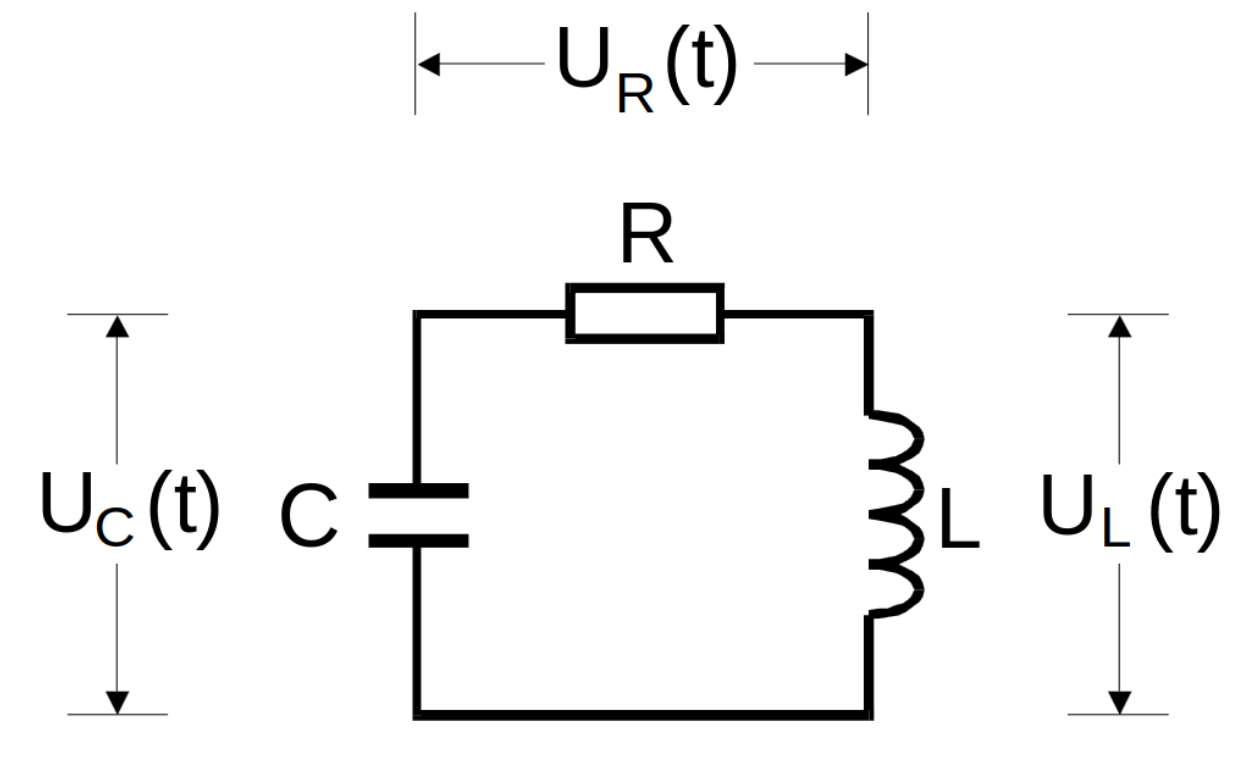
\includegraphics[width=0.5\linewidth]{Gedaempfter_Schwingkreis.png}
    \caption{Schaltbild eines gedämpften Schwingkreises mit Spule, ohmschen Widestand und Kondensator. [Q\cite{anleitungV354}]}
    \label{pic:Gedaempfter_Schwingkreis}
\end{figure}

Das Verhalten des gedämpften Schwingkreises lässt sich durch die Differentialgleichung 
\begin{equation}
    \ddot{I} + \frac{R}{L} \cdot \dot{I} + \frac{1}{L C} \cdot I = 0 
\end{equation}
beschreiben. $I$ ist dabei der im Schwingkreis fließende Strom. 
Diese Gleichung wird durch die Funktion  
\begin{equation}
    I = \symup{e}^{-2\pi\mu t} \cdot \left(\symup{B}_1 \cdot \symup{e}^{2\pi\nu \symup{i}t}  + \symup{B}_2 \cdot \symup{e}^{- 2\pi\nu \symup{i}t} \right)
\end{equation}
gelöst. Für diese Funktion werden die Abkürzungen 
\begin{equation*}
2 \pi \mu \coloneqq \frac{R}{2 L}  \,\,\text{und}\,\, 2 \pi \nu \coloneqq \sqrt{\frac{1}{LC} - \left(\frac{R}{2L}\right)²}
\end{equation*}
verwendet. Für das Verhalten der Schwingung ist entscheident, ob $\nu$ eine imaginäre
oder reelle Zahl ist. Dies hängt davon ab in welchem Größenverhältnis die beiden 
Summanden unter der Wurzel stehen. \\
\\
\textbf{1. Schwingfall}\\
Damit der Schwingfall eintritt, in dem die Amplitude harmonisch mit einer bestimmten Frequenz 
oszilliert, während sie sich auf den 
Nullpunkt zubewegt, muss $\nu$ eine reelle Zahl sein. Dies wird erfüllt, wenn 
\begin{equation*}
    \frac{1}{LC} > \left(\frac{R}{2L}\right)² 
\end{equation*}
gilt. Die Funktion von $I$ vereinfacht sich in diesem Fall zu
\begin{equation}
    I = \symup{A}_0 \cdot \symup{e}^{-2\pi\mu t} \cdot \cos{ \left(2\pi\nu t + \eta\right)} \, .
\end{equation}
$\symup{A}_0$ und $\eta$ sind reelle Konstanten. Die Abklingdauer $T_{\text{ex}}$ der Amplitude bezeichnet
die Zeit, die benötigt wird, damit die Amplitude auf den $\symup{e}$-ten Teil des 
ursprünglichen Wertes abgenommen hat. Für die Abklingdauer gilt
\begin{equation}
    T_{\text{ex}} = \frac{1}{2\pi\mu} = \frac{2 L}{R} \, .
    \label{eqn:Abklingzeit}
\end{equation}
Die einhüllende Funktion zur gedämpften Schwingung ist die Funktion $\pm \symup{e}^{-2\pi\mu t}$. \\
\\
\textbf{2. Kriechfall}\\
Der Kriechfall tritt ein, wenn eine aperiodische Dämpfung vorliegt, wodurch
 $\nu$ eine imaginäre Zahl ist, welche durch 
\begin{equation*}
    \frac{1}{LC} < \left(\frac{R}{2L}\right)² 
\end{equation*}
zustandekommt. Die Lösungsfunktion von $I$ enthält nun keinen oszillierenden Anteil mehr. 
Abhängig von der Wahl der Konstanten $\symup{B}_1$ und $\symup{B}_2$ erreicht $I$ zu Beginn ein Extremwert 
oder geht direkt monoton auf den Nullpunkt zu. Kriechfälle für verschiedene Konstanten 
sind als durchgezogene, farbige Striche in Abbildung (\ref{pic:aperiodische_Daempfung})
dargestellt. 
Für große Zeiten gilt
\begin{equation*}
    I \sim \symup{e}^{- 2\pi \left(\mu - \nu \symup{i}\right)t}\, . 
\end{equation*}
 \\
\textbf{3. Aperiodischer Grenzfall}\\
Der aperiodische Grenzfall ist ein Spezialfall in dem $I$ am schnellsten gegen den 
Nullpunkt geht. 
Für diesen Fall gilt 
\begin{equation}
    \frac{1}{LC} = \left(\frac{R}{2L}\right)² \, .
    \label{eqn:aperiodischerGrenzfall}
\end{equation}
Daraus folgt, dass $\nu = 0$ ist. Die Funktion $I$ vereinfacht sich zu
\begin{equation*}
    I = \symup{D} \cdot \symup{e}^{- \frac{t}{\sqrt{L C}}} \, .
\end{equation*} 
$\symup{D}$ ist eine reelle Konstante. In Abbildung (\ref{pic:aperiodische_Daempfung})
ist der aperiodische Grenzfall als gestrichelte, schwarze Linie dargestellt. 

\begin{figure}[H]
    \centering
    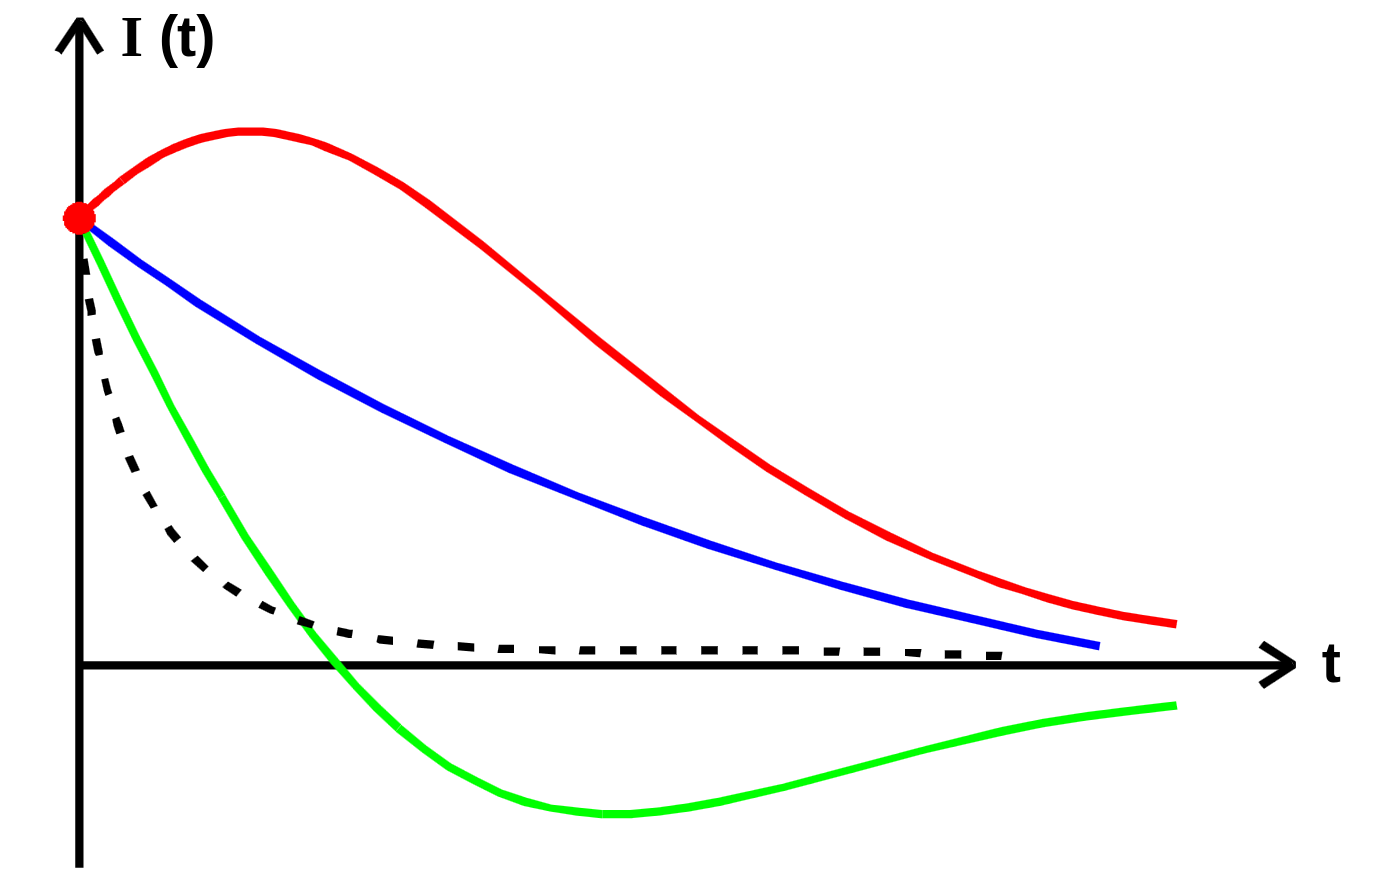
\includegraphics[width=0.7\linewidth]{Aperiodische_Daempfung_Abbildung.png}
    \caption{Verhalten von Strom $I$ in einem Schwingkreis bei aperiodischer Dämpfung. [Q\cite{anleitungV354}]}
    \label{pic:aperiodische_Daempfung}
\end{figure}

\subsection{Erzwungene Schwingungen}
In einem Schwingkreis entsteht eine erzwungene Schwingung, wenn dieser eine äußere 
periodische Krafteinwirkung erfährt. In diesem Fall ist die Kraft eine Spannungsquelle
mit sinusförmiger Wechselspannung $U(t)$. Dieser Schwingkreis ist in Abbildung 
(\ref{pic:erzwungene_Schwingung_Schwingkreis}) zu sehen. 

\begin{figure}[H]
    \centering
    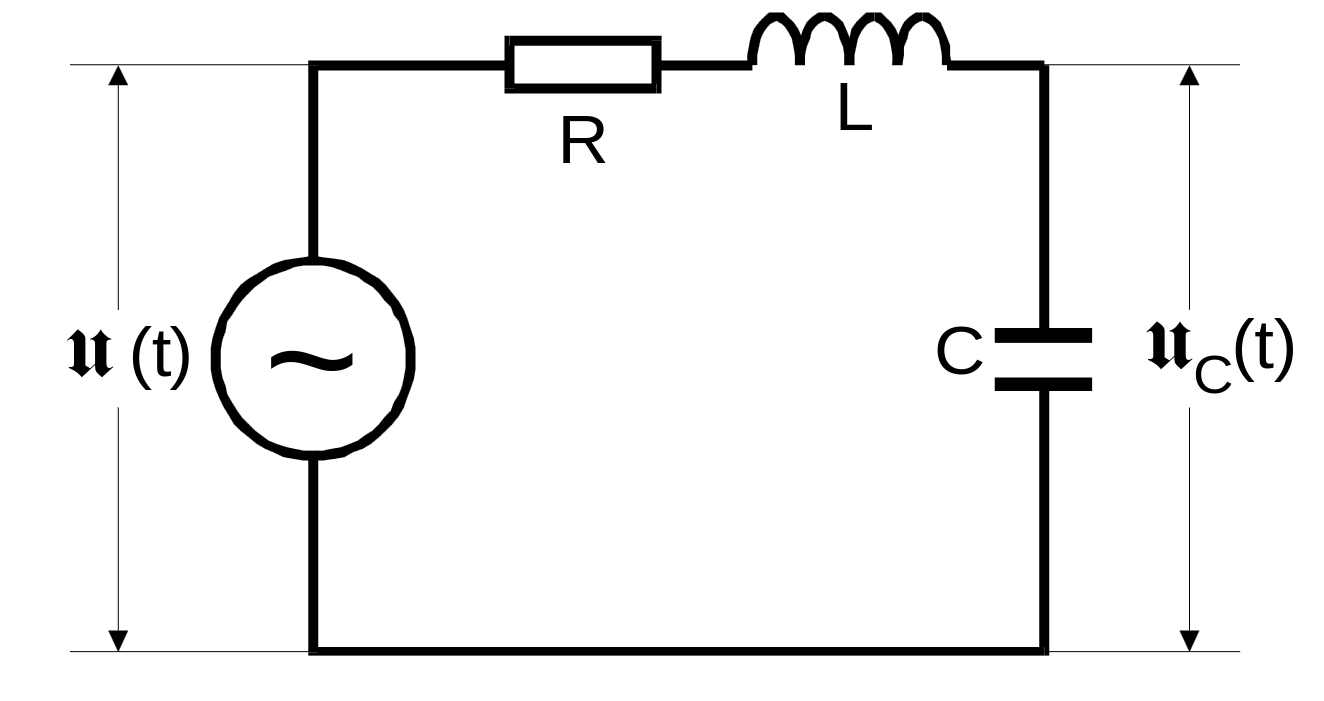
\includegraphics[width=0.5\linewidth]{erzwungene_Schwingung_Schwingkreis.png}
    \caption{Schwingkreis an dem eine sinusförmige Wechselstromquelle angeschlossen ist. [Q\cite{anleitungV354}]}
    \label{pic:erzwungene_Schwingung_Schwingkreis}
\end{figure}

Die Differentialgleichung 
\begin{equation}
    \label{eqn:diffgleichung_erzwungene_Schwingung}
    LC \cdot \ddot{U}_{\text{C}} + RC \cdot \dot{U}_{\text{C}} + U_{\text{C}} = \symup{U}_0 \cdot \symup{e}^{\omega \symup{i} t}
\end{equation}
beschreibt das System. $\symup{U}_0$ ist eine Konstante. Diese Gleichung wird durch den Ansatz $U_{\text{C}} = U \cdot \symup{e}^{\omega \symup{i}t}$ mit
\begin{equation}
    U = \frac{\symup{U}_0 \cdot \left(1 - LC \omega² - \omega R C \symup{i}\right)}{\left(1 - LC \omega²\right)² + \omega² R² C²}
\end{equation}
gelöst. Der Betrag von $U$ beträgt 
\begin{equation}
    |U| = \symup{U}_0 \sqrt{\frac{\left(1 - LC \omega²\right)² + \omega² R² C²}{\left(\left(1 - LC\omega²\right)² + \omega² R² C²\right)²}} 
\end{equation}
und die Phase ist
\begin{equation}
    \varphi (\omega) = \arctan{\left(\frac{- \omega R C}{1 - L C \omega²} \right)}. 
\end{equation}
Die Funktion 
\begin{equation}
    U_{\text{C}}(\omega) = \frac{\symup{U}_0}{\sqrt{\left(1 - LC \omega²\right)² + \omega² R² C²}}
    \label{eqn:Theoriekurve}
\end{equation}
löst die Differentialgleichung (\ref{eqn:diffgleichung_erzwungene_Schwingung}).
$U_{\text{C}}(\omega)$ hat ein Maximum für die Resonanzfrequenz $\omega_{\text{res}}$.
Diese beträgt
$$\omega_{\text{res}} = \sqrt{\frac{1}{LC} - \frac{R²}{2L²}}\, .$$
Für $\omega \rightarrow 0$ und $\omega \rightarrow \infty$ strebt $U_{\text{C}}(\omega)$
gegen die Erregeramplitude $\symup{U}_{\text{0}}(\omega)$.
Für den Fall der schwachen Dämpfung, für den 
$$\frac{R²}{2L²} << \frac{1}{LC}$$
gilt, nähert sich $\omega_{\text{res}}$ der Frequenz $\omega_0$ von der ungedämpften Schwingung an. 
In diesem Fall wird das Maximum von $U_{\text{C}}$ durch 
$$U_{\text{C,max}} =  \frac{1}{\omega_0 R C} \cdot \symup{U}_0 = \frac{1}{R}\sqrt{\frac{L}{C}} \, \symup{U}_0$$
ausgedrückt. 
Falls $R \rightarrow 0$ geht $U_{\text{C,max}} \rightarrow \infty$. Der Vorfaktor 
$\frac{1}{\omega_0 R C}$ heißt Resonanzüberhöhung oder auch Güte $q$ des Schwingkreises.
Die Breite der Resonanzkurve wird mithilfe der Frequenzen $\omega_+$ und $\omega_-$ beschrieben, 
bei denen 
$$U_{\text{C}}(\omega_{+,-}) = \frac{1}{\sqrt{2}} \cdot U_{\text{C,max}}$$
gilt. Unter der Voraussetzung, dass 
$$\frac{R²}{L²} << \omega²_0$$
gilt, wird die Breite der Resonanzkurve durch 
\begin{equation}
\omega_+ - \omega_- \thickapprox \frac{R}{L}
\label{eqn:BreiteResonanzkurve}
\end{equation}
ausgedrückt.
Die Güte $q$ wird ausgedrückt durch
\begin{equation}
    q = \frac{\omega_0}{\omega_+ - \omega_- } \, .
    \label{eqn:Güte}
\end{equation}